%

\providecommand{\imwidth}{}

\providecommand{\impath}[1]{}
\providecommand{\impaths}[1]{}
\providecommand{\impatha}[1]{}
\providecommand{\impathb}[1]{}
\providecommand{\impathc}[1]{}
\providecommand{\impathd}[1]{}
\providecommand{\impathe}[1]{}


\newcommand{\convolutionalcows}{
\begin{figure}[!t]
	\centering
   \includegraphics[width=0.48\textwidth]{img/cowsample}
\caption{Convolutional Cows.}
\end{figure}
}

\newcommand{\perceptualcompression}{
\begin{figure}[!t]
	\centering
   \includegraphics[width=0.38\textwidth]{img/generativevscompressive4}
\caption{\label{fig:perceptualcompression}
%
%
%
%
%
%
%
%
%
%
Illustrating perceptual and semantic compression: Most bits of a digital image correspond to imperceptible details. While DMs allow to suppress this semantically meaningless information by minimizing the responsible loss term, gradients (during training) and the neural network backbone (training and inference) still need to be evaluated on all pixels, leading to superfluous computations and unnecessarily expensive optimization and inference.
\\
We propose \emph{latent diffusion models (LDMs)} as an effective generative model and a separate mild compression stage that only eliminates imperceptible details.
Data and images from \cite{DBLP:conf/nips/HoJA20}.\vspace{-1.25em}
%
}
\end{figure}
}

\newcommand{\churchesdiscretevscont}{
\begin{figure}[htbp]
	\centering
   \includegraphics[width=0.48\textwidth]{img/contvsdiscrete/fids_f4churches}
   \includegraphics[width=0.48\textwidth]{img/contvsdiscrete/is_f4churches}
\caption{FID and IS on LSUN-Churches vs training iterations, evaluated on 2k samples.}
\end{figure}
}


%
%
%
%
%
%
%
%

\newcommand{\crossattnfig}{
\begin{figure}[tbp]
\centering
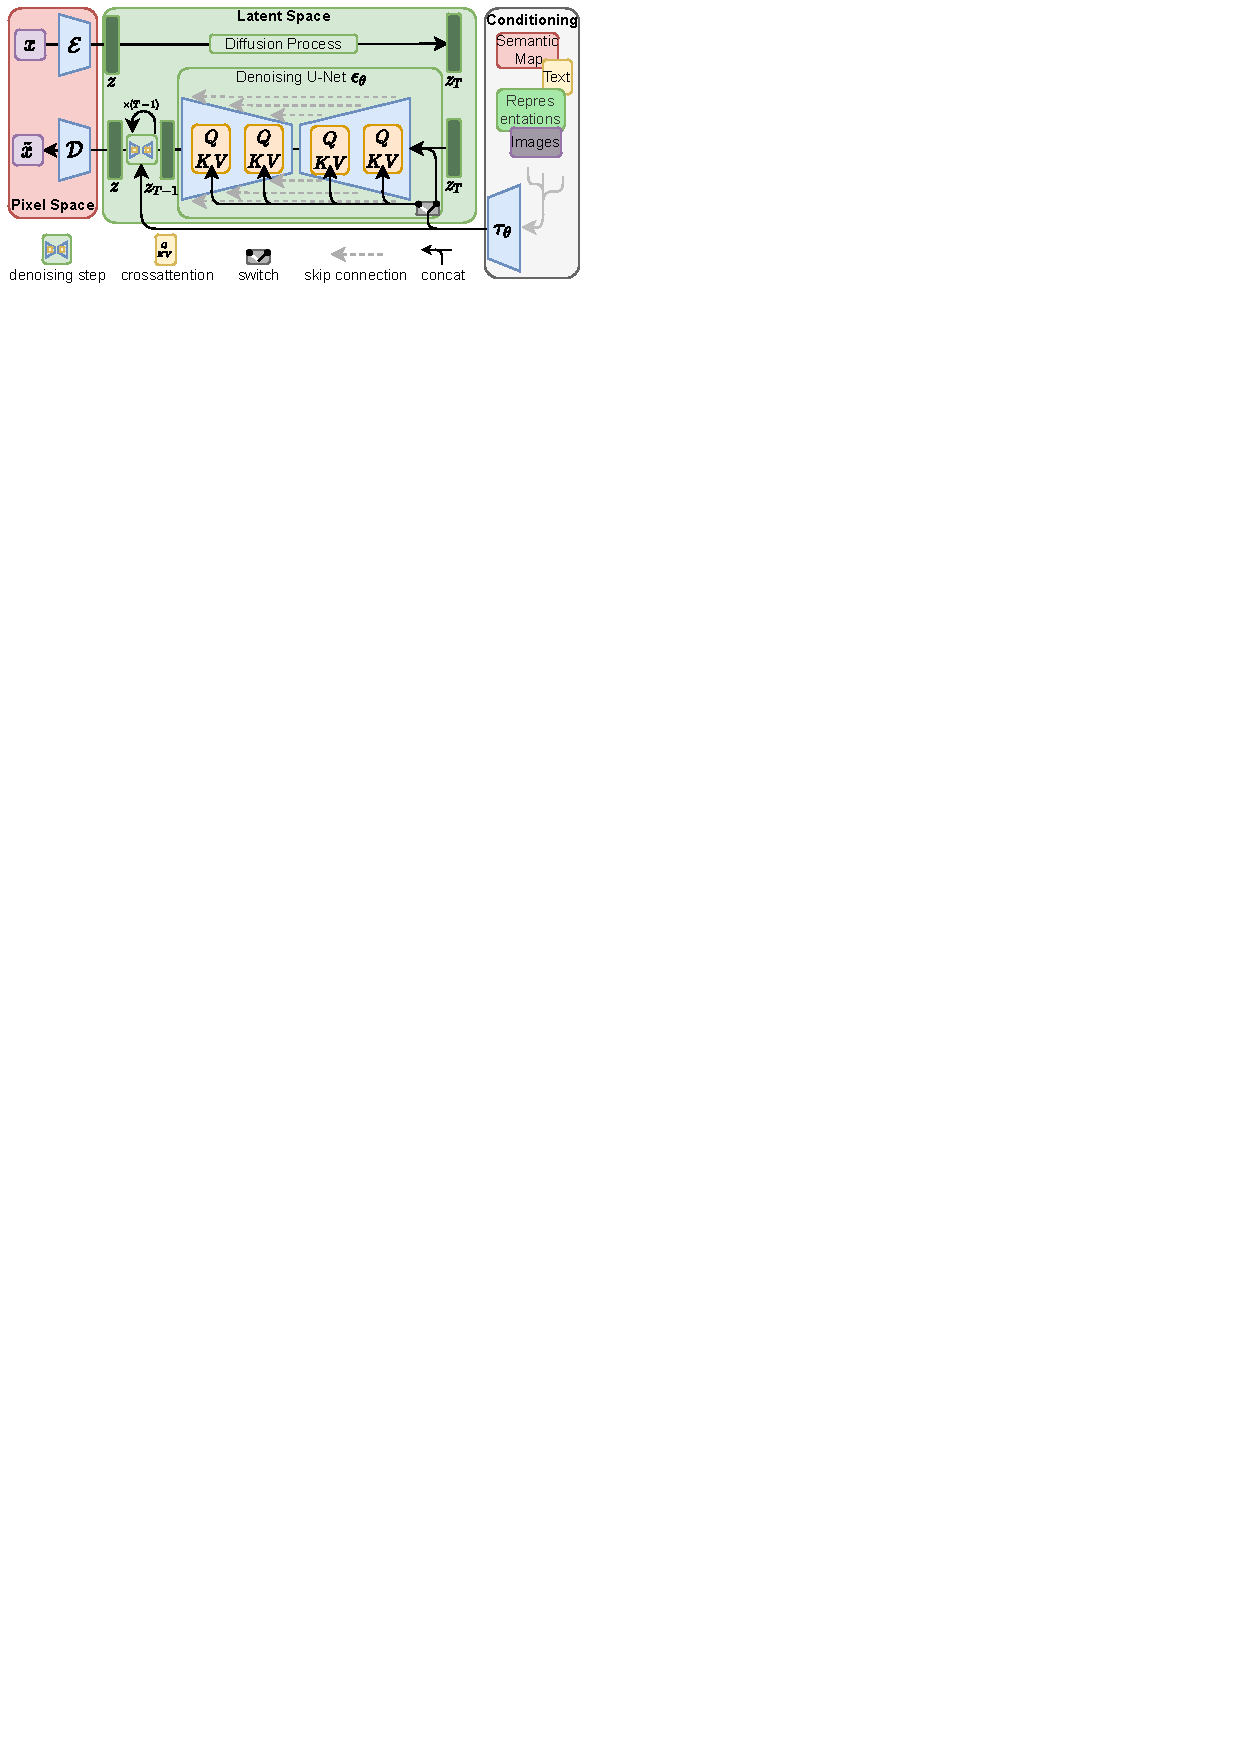
\includegraphics[trim=0 705 305 2, clip, width=0.5\textwidth]{img/final_figure.pdf}
  \caption{\label{fig:conditioning} We condition LDMs either via concatenation %
  or by a more general cross-attention mechanism. See Sec.~\ref{subsec:conditioning} \vspace{-1.5em}}
\end{figure}
}

\newcommand{\thicksample}{
\begin{figure}[htbp]
\centering
\includegraphics[width=0.5\textwidth]{img/highlandscapes/goodersample}\vspace{-0.65em}
  \caption{\label{fig:thicksample} A \emph{LDM} trained on $256^2$ resolution can generalize to 
  larger resolution (here: $512\times1024$) for spatially conditioned tasks
  such as semantic synthesis of landscape images. See
  Sec.~\ref{subsubsec:beyond}.\vspace{-1em}
  }
\end{figure}
}


\newcommand{\cincompression}{
\begin{figure}[htbp]
\begin{subfigure}{.275\textwidth}
\centering
   \includegraphics[width=\linewidth]{img/compression_analysis/fid_vs_trainstep_cin_new2}
\end{subfigure}
\hfill
\begin{subfigure}{.195\textwidth}
\centering
\includegraphics[width=\linewidth]{img/compression_analysis/is_vs_trainstep_cin_new2}
\end{subfigure}
\caption{\label{fig:cin_traincourse}Analyzing the training of class-conditional \emph{LDMs} with different downsampling factors $f$ over 2M train steps on the ImageNet dataset. 
%
Pixel-based \emph{LDM-1}
requires substantially larger train times compared to models with larger downsampling factors (\emph{LDM-$\{$4-16$\}$}). 
Too much perceptual compression as in \emph{LDM-32} limits the overall sample quality.
All models are trained on a single NVIDIA A100 with the same computational budget. 
Results obtained with 100 DDIM steps~\cite{DBLP:conf/iclr/SongME21} and $\kappa = 0$.\vspace{-1em} }
\end{figure}
}

\newcommand{\cifarfirststagemetrics}{
\begin{figure*}[htbp]
	\centering
   \includegraphics[width=0.48\textwidth]{img/first_stage_models/cifar_psim_and_ssim}
   \includegraphics[width=0.48\textwidth]{img/first_stage_models/cifar_recfid_and_psnr}
\caption{Reconstruction metrics as a function of codebook size, evaluated on CIFAR-10 val.}
\end{figure*}
}

\newcommand{\vqganfirststagemetrics}{
\begin{figure*}[htbp]
	\centering
   \includegraphics[width=0.48\textwidth]{img/first_stage_models/vqgan_psim_and_ssim}
   \includegraphics[width=0.48\textwidth]{img/first_stage_models/vqgan_rfid_and_psnr}
\caption{Reconstruction metrics as a function of compression ratio, evaluated on ImageNet val.}
\end{figure*}
}

\newcommand{\cindiscretevscont}{
\begin{figure}[htbp]
	\centering
   \includegraphics[width=0.48\textwidth]{img/contvsdiscrete/fids_and_is_over_ddim_cin_1m}
\caption{\label{fig:cindiscretevscont} Sampling of continuous and discrete models trained on class-conditional ImageNet (256) for different numbers of function evaluations (DDIM sampling). Evaluated on 50000 (?) samples. Both models trained for 1M steps. \todo{add rec-fid}. Note: $\kappa=1.0$, $f=4$}
\end{figure}
}

\newcommand{\sflckrdiscretevscont}{
\begin{figure}[htbp]
	\centering
   \includegraphics[width=0.48\textwidth]{img/contvsdiscrete/cont_vs_vq_f4_sflckr}
\caption{\label{fig:sflckrdiscretevscont} Sampling of continuous and discrete models trained SFLCKR (256) for different numbers of function evaluations (DDIM sampling). Evaluated on val split (approx. 14k examples). Both models trained for 1M steps. \todo{add rec-fid}. Note: $\kappa=1.0$, $f=4$}
\end{figure}
}


\newcommand{\firststagecomparison}{
\begin{figure}[thbp]
	\centering
	%
    \renewcommand{\imwidth}{0.5\textwidth}
    \renewcommand{\impaths}[1]{img/firststagereconstructions/new/##1} 
    \setlength{\tabcolsep}{1pt}
    \renewcommand{\arraystretch}{1}
	\begin{adjustbox}{max width=\linewidth} %
 	\begin{tabular}{c c c c}
  	\toprule
  	\Huge \textbf{Input} & \shortstack{\Huge \textbf{ours ($f=4$)} \\ \huge
    PSNR: $27.4$ R-FID: $0.58$} &  \shortstack{\Huge \textbf{DALL-E ($f=8$)}
    \\ \huge PSNR: $22.8$ R-FID: $32.01$}  & \shortstack{\Huge \textbf{VQGAN
    ($f=16$)} \\ \huge PSNR: $19.9$ R-FID: $4.98$}\\
  	\midrule
	\includegraphics[width=\imwidth]{\impaths{up1}} &	         
		\includegraphics[width=\imwidth]{\impaths{up2}} &	         
			\includegraphics[width=\imwidth]{\impaths{up3}} &	         
				\includegraphics[width=\imwidth]{\impaths{up4}} \\
				
%
%
%
%
				
	\includegraphics[width=\imwidth]{\impaths{down1}} &	         
		\includegraphics[width=\imwidth]{\impaths{down2}} &	         
			\includegraphics[width=\imwidth]{\impaths{down3}} &	         
				\includegraphics[width=\imwidth]{\impaths{down4}} \\	         
  	\bottomrule
	\end{tabular}
	\end{adjustbox}
	\caption{\label{fig:firststagecomparison} Boosting the upper bound on achievable quality with less agressive downsampling.
	Since diffusion models offer excellent inductive biases for spatial data, we do not need the heavy spatial downsampling of related generative models in latent space, but can still greatly reduce the dimensionality of the data via suitable autoencoding models, see Sec.~\ref{sec:method}.
%
	Images are from the DIV2K \cite{DBLP:conf/cvpr/AgustssonT17} validation set, evaluated at $512^2$ px. We denote the spatial
	downsampling factor by $f$. Reconstruction FIDs %
	\cite{FID} and PSNR are calculated on ImageNet-val. \cite{DBLP:conf/cvpr/DengDSLL009}; 
%
	see also Tab.~\ref{tab:firststagetablecomplete}.
	} \vspace{-1.25em}
\end{figure}
}


\newcommand{\celebadiscretevscontqualitative}{
\begin{figure*}[thbp]
	\centering
	%
    \renewcommand{\imwidth}{0.5\textwidth}
    \renewcommand{\impaths}[1]{img/contvsdiscrete/celeba/##1} 
    \setlength{\tabcolsep}{1pt}
    \renewcommand{\arraystretch}{1}
	\begin{small}
	\begin{adjustbox}{max width=\linewidth, totalheight=\textheight-2\baselineskip}
 	\begin{tabular}{c cc}
  	\toprule
  	DDIM steps & VQ $f_4$ & VAE $f_4$ \\
  	\midrule
  	5 & 
	\includegraphics[width=\imwidth]{\impaths{vq_5_steps}} &	         
    \includegraphics[width=\imwidth]{\impaths{cont_5_steps}} \\
    
  	10 & 
	\includegraphics[width=\imwidth]{\impaths{vq_10_steps}} &	         
    \includegraphics[width=\imwidth]{\impaths{cont_10_steps}} \\

  	20 & 
	\includegraphics[width=\imwidth]{\impaths{vq_20_steps}} &	         
    \includegraphics[width=\imwidth]{\impaths{cont_20_steps}} \\
 
   	50 & 
	\includegraphics[width=\imwidth]{\impaths{vq_50_steps}} &	         
    \includegraphics[width=\imwidth]{\impaths{cont_50_steps}} \\
    
    100 & 
	\includegraphics[width=\imwidth]{\impaths{vq_100_steps}} &	         
    \includegraphics[width=\imwidth]{\impaths{cont_100_steps}} \\
    
    200 & 
	\includegraphics[width=\imwidth]{\impaths{vq_200_steps}} &	         
    \includegraphics[width=\imwidth]{\impaths{cont_200_steps}} \\
  	\bottomrule
	\end{tabular}
	\end{adjustbox}
	\end{small}
	\caption{\label{fig:celebadiscretevscontqualitative} Qualitative assessment of the differences of continuous and discrete first stages, evaluated on CelebA. $\kappa=1.0$, settings as in Fig.~\ref{fig:celebadiscretevscont}. Random Samples.}
\end{figure*}
}

\newcommand{\imagenetsamples}{
\begin{figure*}[thbp]
	\centering
	%
    \renewcommand{\imwidth}{.9\textwidth}
    \renewcommand{\impaths}[1]{img/goodsamples/cin_samples/##1} 
    \setlength{\tabcolsep}{1pt}
    \renewcommand{\arraystretch}{1}
	\begin{small}
%
 	\begin{tabular}{c c}
  	\toprule
%
%
  	c156 & 	         
    \includegraphics[width=\imwidth]{\impaths{blenheim_spanial_row}} \\
    
  	c992 & 	         
    \includegraphics[width=\imwidth]{\impaths{c992-agaric_row}} \\
	
c292 & 
    \includegraphics[width=\imwidth]{\impaths{c291_lion_row}} \\
 	
	
  	c292 & 
    \includegraphics[width=\imwidth]{\impaths{c90_lorikeet_row}} \\
 
   	c963 &       
    \includegraphics[width=\imwidth]{\impaths{c963_pizza_row2}} \\
    
    c417& 	         
    \includegraphics[width=\imwidth]{\impaths{c417_ballon_row}} \\
    
    200 & 
    \includegraphics[width=\imwidth]{\impaths{c323-monarch_butterfly_row}} \\
  	\bottomrule
	\end{tabular}
%
	\end{small}
	\caption{\label{fig:imagenetsamples} Random Samples of our f-4 guided imagenet model.}
\end{figure*}
}

\newcommand{\celebaprogrows}{
\begin{figure*}[th]
	\centering
	%
    \renewcommand{\imwidth}{0.5\textwidth}
    \renewcommand{\impaths}[1]{img/contvsdiscrete/celeba/##1} 
    \setlength{\tabcolsep}{1pt}
    \renewcommand{\arraystretch}{1}
	\begin{small}
	\begin{adjustbox}{max width=\linewidth, totalheight=\textheight-2\baselineskip}
 	\begin{tabular}{l c}
  	\toprule
  	Model & Samples \\
  	\midrule
  	VQ $f_4$ & 
	\includegraphics[width=\imwidth]{\impaths{vq_prog_row_ddpm}} \\
    
    VQ $f_4$ w/ $q(z_0)$ & 
	\includegraphics[width=\imwidth]{\impaths{vq_prog_row_x0q_ddpm}} \\
	
  	VAE $f_4$ & 
	\includegraphics[width=\imwidth]{\impaths{vae_prog_row_ddpm}} \\
  	\bottomrule
	\end{tabular}
	\end{adjustbox}
	\end{small}
	\caption{\label{fig:celebaprogrows} Progressive decoding for vanilla DDPM sampling (1000 steps) on CelebA. Random Samples.}
\end{figure*}
}

\newcommand{\speeeeed}{
\begin{figure}[thbp]
\begin{subfigure}{.275\textwidth}
\centering
   \includegraphics[width=\linewidth]{img/speed_vs_fid/celeba-complete_new2}
\end{subfigure}
\hfill
\begin{subfigure}{.195\textwidth}
\centering
\includegraphics[width=\linewidth]{img/speed_vs_fid/cin-complete_new2}
\end{subfigure}
\caption{\label{fig:speedplot} Comparing
  \emph{LDMs} with varying compression on the CelebA-HQ (left) and
  ImageNet (right) datasets. Different markers indicate $\{10, 20, 50, 100,
  200\}$ sampling steps using DDIM, from right to left along
  each line. The dashed line shows the FID scores for 200 steps, indicating the
  strong performance of \emph{LDM-$\{$4-8$\}$}.
%
  FID scores assessed on 5000 samples. All models
  were trained for 500k (CelebA) / 2M (ImageNet) steps on an A100.\vspace{-2em}
}
\end{figure}
}


\newcommand{\celebalosscomp}{
\begin{figure}[htbp]
	\centering
   \includegraphics[width=0.48\textwidth]{img/lvlb_vs_lsimple/frechet_inception_distance}
\caption{\label{fig:celebalosscomp} Comparinfg LVQ-diffusion models trained on CelebAHQ with $\mathcal{L}_{\mathrm{simple}}$ (blue) and $\mathcal{L}_{\mathrm{vlb}}$ (orange) in terms of FID when sampling 50 steps with DDIM. Results indicate that, also in quantized feature spaces, it is beneficial to train with the reweighted objective $\mathcal{L}_{\mathrm{simple}}$.  Note: $\kappa=0.0$, $f=4$}
\end{figure}
}

\newcommand{\bboxtoimgsamples}{
\begin{figure}[htbp]
\hfill
\parbox[b]{.5\textwidth}{
\centering
\small
	\renewcommand{\imwidth}{0.08\textwidth}
    \renewcommand{\impatha}[1]{img/goodsamples/bbox2img/street/##1} 
	\renewcommand{\impathb}[1]{img/goodsamples/bbox2img/table/##1} 
    \renewcommand{\impathc}[1]{img/goodsamples/bbox2img/surfer/##1}
	\setlength{\tabcolsep}{0pt}
	%
	\begin{tabular}{c@{\hskip 2pt}ccccc}
	\toprule
	\multicolumn{6}{c}{Layout-to-Image Synthesis evaluated on COCO~\cite{DBLP:conf/cvpr/CaesarUF18}}\\	
	\midrule
	\includegraphics[align=c,width=\imwidth]{\impatha{cond-2_}} &	         
	\includegraphics[align=c,width=\imwidth]{\impatha{sample-176}} &	        
	\includegraphics[align=c,width=\imwidth]{\impatha{sample-216}} &	
	\includegraphics[align=c,width=\imwidth]{\impatha{sample-251}} &	        
	\includegraphics[align=c,width=\imwidth]{\impatha{sample-439}} &  
    \includegraphics[align=c,width=\imwidth]{\impatha{sample-266}} \\
    \rule{0pt}{6ex}%
    \includegraphics[align=c,width=\imwidth]{\impathb{cond-185_}} &	         
	\includegraphics[align=c,width=\imwidth]{\impathb{sample-219}} &	        
	\includegraphics[align=c,width=\imwidth]{\impathb{sample-319}} &	
	\includegraphics[align=c,width=\imwidth]{\impathb{sample-249}} &	        
	\includegraphics[align=c,width=\imwidth]{\impathb{sample-259}} &  
    \includegraphics[align=c,width=\imwidth]{\impathb{sample-199}} \\
    \rule{0pt}{6ex}%
    \includegraphics[align=c,width=\imwidth]{\impathc{cond-1_}} &	         
	\includegraphics[align=c,width=\imwidth]{\impathc{sample-36}} &	        
	\includegraphics[align=c,width=\imwidth]{\impathc{sample-39}} &	
	\includegraphics[align=c,width=\imwidth]{\impathc{sample-48}} &	        
	\includegraphics[align=c,width=\imwidth]{\impathc{sample-434}} &  
    \includegraphics[align=c,width=\imwidth]{\impathc{sample-398}} \\
	
	\bottomrule
    \end{tabular}

}
\caption{\label{fig:bbox2img} Samples from our model for complex scene synthesis on the COCO~\cite{DBLP:conf/cvpr/CaesarUF18} dataset. For more samples and also quantitative results /cf the supplement.}
\end{figure}
}


\newcommand{\bboxandtexttoimgsamples}{
%
\begin{figure}[tbp]
\centering
%
\parbox[b]{.5\textwidth}{
\small
	\renewcommand{\imwidth}{0.09\textwidth}
    \renewcommand{\impath}[1]{img/supplement/layouts/##1}%
    \renewcommand{\impathd}[1]{img/cr/text2img/##1}%
    \renewcommand{\impatha}[1]{img/goodsamples/bbox2img/street/##1} 
	\renewcommand{\impathb}[1]{img/goodsamples/bbox2img/table/##1} 
    \renewcommand{\impathc}[1]{img/goodsamples/bbox2img/surfer/##1}
%
    \renewcommand{\impathe}[1]{img/goodsamples/text2img/sunrise/##1} 
	\setlength{\tabcolsep}{0pt}
	%
	\begin{tabular}{c@{\hskip 2pt}cccc}
	\toprule
	%
	%
	\includegraphics[align=c,width=\imwidth]{\impatha{cond-2_}} &	         
%
	\includegraphics[align=c,width=\imwidth]{\impatha{sample-216}} &	
	\includegraphics[align=c,width=\imwidth]{\impatha{sample-251}} &	        
	\includegraphics[align=c,width=\imwidth]{\impatha{sample-439}} &  
    \includegraphics[align=c,width=\imwidth]{\impatha{sample-266}} \\
    \rule{0pt}{5ex}%
%
%
%
%
%

	\includegraphics[align=c,width=\imwidth]{\impath{train/cond-283}} &
	\includegraphics[align=c,width=\imwidth]{\impath{train/sample-270}} &
	\includegraphics[align=c,width=\imwidth]{\impath{train/sample-330}} &
	\includegraphics[align=c,width=\imwidth]{\impath{train/sample-390}} &
	\includegraphics[align=c,width=\imwidth]{\impath{train/sample-282}} \\
    \rule{0pt}{5ex}%
	\includegraphics[align=c,width=\imwidth]{\impath{flower/cond-99}} &
	\includegraphics[align=c,width=\imwidth]{\impath{flower/sample-98}} &
	\includegraphics[align=c,width=\imwidth]{\impath{flower/sample-134}} &
	\includegraphics[align=c,width=\imwidth]{\impath{flower/sample-158}} &
	\includegraphics[align=c,width=\imwidth]{\impath{flower/sample-206}}\\
	\midrule
	%
	%
%
%
%
%
%
%
    
%
%
%
%
%
%
%
%
%
%
%
%
%
%
%
%
%
%
%
%
	\bottomrule
  \end{tabular}\vspace{-0.5em}
}
\caption{\label{fig:bboxandtxt2img} Layout-to-image synthesis with an \emph{LDM} on COCO~\cite{DBLP:conf/cvpr/CaesarUF18}, see Sec.~\ref{subsubsec:crossattn2img}. Quantitative evaluation in the supplement \ref{suppsec:bboxtoimage}. 
%
 \vspace{-1em}}
\end{figure}
}


\newcommand{\texttoimgsamples}{
\begin{figure}[htbp]
\hfill
\parbox[b]{.5\textwidth}{
\centering
\small
    \renewcommand{\imwidth}{0.12\textwidth}
    \renewcommand{\impatha}[1]{img/goodsamples/text2img/sunrise/##1} 
	\renewcommand{\impathb}[1]{img/goodsamples/text2img/flowers/##1} 
    \renewcommand{\impathc}[1]{img/goodsamples/text2img/dog_puppy/##1} 
    \renewcommand{\impathd}[1]{img/goodsamples/text2img/crowded/##1} 
	\setlength{\tabcolsep}{0pt}
	\begin{tabular}{c@{\hskip 2pt}c@{\hskip 2pt}c@{\hskip 2pt}c}
	\toprule
	\footnotesize{\emph{'Sunset over}} & \footnotesize{\emph{'Flowers on a}} & \footnotesize{\emph{'A dog}} & \footnotesize{\emph{'A crowded scene}}  \\
    \footnotesize{\emph{an old town.'}} & \footnotesize{\emph{field in spring.'}} & \footnotesize{\emph{puppy.'}} & \footnotesize{\emph{in front of a pub.'}} \\
    \midrule
	\includegraphics[align=c,width=\imwidth]{\impatha{sample-200}} &	         
	\includegraphics[align=c,width=\imwidth]{\impathb{sample-159}} &	        
	\includegraphics[align=c,width=\imwidth]{\impathc{sample-484}} &	  
    \includegraphics[align=c,width=\imwidth]{\impathd{sample-71}} \\
    
    \includegraphics[align=c,width=\imwidth]{\impatha{sample-180}} &	         
	\includegraphics[align=c,width=\imwidth]{\impathb{sample-169}} &	        
	\includegraphics[align=c,width=\imwidth]{\impathc{sample-801}} &	  
    \includegraphics[align=c,width=\imwidth]{\impathd{sample-87}} \\
    
    \includegraphics[align=c,width=\imwidth]{\impatha{sample-120}} &	         
	\includegraphics[align=c,width=\imwidth]{\impathb{sample-209}} &	        
	\includegraphics[align=c,width=\imwidth]{\impathc{sample-1080}} &	  
    \includegraphics[align=c,width=\imwidth]{\impathd{sample-167}} \\
    
    \includegraphics[align=c,width=\imwidth]{\impatha{sample-150}} &	         
	\includegraphics[align=c,width=\imwidth]{\impathb{sample-239}} &	        
	\includegraphics[align=c,width=\imwidth]{\impathc{sample-1223}} &	  
    \includegraphics[align=c,width=\imwidth]{\impathd{sample-201}} \\
    \bottomrule
    \end{tabular}
}
\caption{\label{fig:text2img} Samples from our text-to-image model for user-defined text prompts. Our model is pretrained on the LAION~\cite{schuhmann2021laion400m} database and finetuned on the Conceptual Captions\cite{sharma2018conceptual} dataset.}
\end{figure}
}
	
	

\newcommand{\smallsamples}{
\begin{figure*}[htbp]
\hfill%
  \parbox[b]{\textwidth}{
\centering
\small
    \renewcommand{\imwidth}{0.065\textwidth}
    \renewcommand{\impatha}[1]{img/goodsamples/celeba/##1} 
	\renewcommand{\impathb}[1]{img/goodsamples/ffhq/##1} 
    \renewcommand{\impathc}[1]{img/goodsamples/churches/##1} 
    \renewcommand{\impathd}[1]{img/goodsamples/beds/##1} 
    \renewcommand{\impathe}[1]{img/goodsamples/cin_cherries/##1} 
	\setlength{\tabcolsep}{0pt}		
 \begin{tabular}{ccc@{\hskip 2pt}ccc@{\hskip 2pt}ccc@{\hskip 2pt}ccc@{\hskip 2pt}ccc}
    \toprule
 	 \multicolumn{3}{c}{CelebAHQ} & \multicolumn{3}{c}{FFHQ} & \multicolumn{3}{c}{LSUN-Churches} & \multicolumn{3}{c}{LSUN-Beds}& \multicolumn{3}{c}{ImageNet} \\ 
  \toprule
	\includegraphics[align=c,width=\imwidth]{\impatha{sample-7}} &	         
	\includegraphics[align=c,width=\imwidth]{\impatha{sample-10}} &	        
	\includegraphics[align=c,width=\imwidth]{\impatha{sample-11}} &	         
	
	\includegraphics[align=c,width=\imwidth]{\impathb{sample-4}} &	         
	\includegraphics[align=c,width=\imwidth]{\impathb{sample-5}} &	        
	\includegraphics[align=c,width=\imwidth]{\impathb{sample-6}} &
	
	\includegraphics[align=c,width=\imwidth]{\impathc{sample-48}} &	         
	\includegraphics[align=c,width=\imwidth]{\impathc{sample-60}} &	        
	\includegraphics[align=c,width=\imwidth]{\impathc{sample-71}} &
	
	\includegraphics[align=c,width=\imwidth]{\impathd{sample-1}} &	         
	\includegraphics[align=c,width=\imwidth]{\impathd{sample-29}} &	        
	\includegraphics[align=c,width=\imwidth]{\impathd{sample-32}} &
	
	\includegraphics[align=c,width=\imwidth]{\impathe{sample-928}} &	         
	\includegraphics[align=c,width=\imwidth]{\impathe{sample-1}} &	        
	\includegraphics[align=c,width=\imwidth]{\impathe{sample-171}} 	
	\\
%
	\includegraphics[align=c,width=\imwidth]{\impatha{sample-18}} &	         
	\includegraphics[align=c,width=\imwidth]{\impatha{sample-23}} &	        
	\includegraphics[align=c,width=\imwidth]{\impatha{sample-32}} &	         
	
	\includegraphics[align=c,width=\imwidth]{\impathb{sample-26}} &	         
	\includegraphics[align=c,width=\imwidth]{\impathb{sample-29}} &	        
	\includegraphics[align=c,width=\imwidth]{\impathb{sample-32}} &
	
	\includegraphics[align=c,width=\imwidth]{\impathc{sample-82}} &	         
	\includegraphics[align=c,width=\imwidth]{\impathc{sample-97}} &	        
	\includegraphics[align=c,width=\imwidth]{\impathc{sample-98}} &
	
	\includegraphics[align=c,width=\imwidth]{\impathd{sample-35}} &	         
	\includegraphics[align=c,width=\imwidth]{\impathd{sample-42}} &	        
	\includegraphics[align=c,width=\imwidth]{\impathd{sample-44}} &
	
	\includegraphics[align=c,width=\imwidth]{\impathe{sample-1042}} &	         
	\includegraphics[align=c,width=\imwidth]{\impathe{sample-48}} &	        
	\includegraphics[align=c,width=\imwidth]{\impathe{sample-116}} 	
	\\	
	\includegraphics[align=c,width=\imwidth]{\impatha{sample-34}} &	         
	\includegraphics[align=c,width=\imwidth]{\impatha{sample-42}} &	        
	\includegraphics[align=c,width=\imwidth]{\impatha{sample-45}} &	         
	
	\includegraphics[align=c,width=\imwidth]{\impathb{sample-45}} &	         
	\includegraphics[align=c,width=\imwidth]{\impathb{sample-49}} &	        
	\includegraphics[align=c,width=\imwidth]{\impathb{sample-51}} &
	
	\includegraphics[align=c,width=\imwidth]{\impathc{sample-103}} &	         
	\includegraphics[align=c,width=\imwidth]{\impathc{sample-104}} &	        
	\includegraphics[align=c,width=\imwidth]{\impathc{sample-116}} &
	
	\includegraphics[align=c,width=\imwidth]{\impathd{sample-47}} &	         
	\includegraphics[align=c,width=\imwidth]{\impathd{sample-49}} &	        
	\includegraphics[align=c,width=\imwidth]{\impathd{sample-53}} &
	
	\includegraphics[align=c,width=\imwidth]{\impathe{sample-287}} &	         
	\includegraphics[align=c,width=\imwidth]{\impathe{sample-71}} &	        
	\includegraphics[align=c,width=\imwidth]{\impathe{sample-128}} 		\\
\bottomrule
\end{tabular}
}
\caption{\label{fig:samples_mix} Samples from \emph{LDMs} trained on CelebAHQ~\cite{DBLP:journals/corr/abs-1710-10196}, FFHQ~\cite{stylegan}, LSUN-Churches~\cite{DBLP:journals/corr/YuZSSX15}, LSUN-Bedrooms~\cite{DBLP:journals/corr/YuZSSX15} and class-conditional ImageNet~\cite{DBLP:conf/cvpr/DengDSLL009}, each with a resolution of $256 \times 256$. Best viewed when zoomed in. For more samples \cf the supplement. \vspace{-1.5em}}
\end{figure*}

}

\newcommand{\mountain}{
\begin{figure*}[htbp]
\hfill%
  \parbox[b]{\textwidth}{
\centering
\small
 \includegraphics[width=0.2\textwidth]{img/sr_images/mountain.jpg}
}
\caption{no capti}
\end{figure*}
}


\newcommand{\testismall}{
\begin{figure*}[htbp]
\hfill%
  \parbox[b]{\textwidth}{
\centering
\small
 \includegraphics[trim=0 512 0 128, clip, width=1.\textwidth]{img/sr_images/mountain.jpg}
}
\caption{no capti}
\end{figure*}
}

\newcommand{\testibig}{
\begin{figure*}[htbp]
\hfill%
  \parbox[b]{\textwidth}{
\centering
\small
 \includegraphics[trim=0 2048 0 512, clip, width=1.\textwidth]{img/sr_images/mountain_sr.jpg}
}
\caption{no capti}
\end{figure*}
}

\newcommand{\testicrop}{
\begin{figure*}[htbp]
\hfill%
  \parbox[b]{\textwidth}{
\centering
\small
 \includegraphics[trim=0 0 0 0, clip, width=1.\textwidth]{img/sr_images/mountain_sr.jpg}
}
\caption{no capti}
\end{figure*}
}

\newcommand{\srmountain}{
\begin{figure}[htbp]
\includegraphics[width = 1.04in]{img/sr_images/mountain.jpg}
\end{figure}
}



%

\newcommand{\srimagenet}{
\begin{figure}[tbp]
%
	\setlength{\tabcolsep}{1.25pt}		
\begin{small}
\begin{tabular}{ccc}
bicubic & \emph{LDM}-SR & SR3 \\
\includegraphics[width = 1.04in]{img/hos/cat_bicubic.jpeg}&
\includegraphics[width = 1.04in]{img/hos/cat_ours_w_box.jpg}&
\includegraphics[width = 1.04in]{img/hos/cat_ho.jpeg}\\
\includegraphics[width = 1.04in]{img/hos/car_bicubic.jpeg}&
\includegraphics[width = 1.04in]{img/hos/car_ours_w_box.jpg}& \includegraphics[width = 1.04in]{img/hos/car_ho.jpeg}\\
\end{tabular}
\end{small}
%
\vspace*{-1.0em}
\caption{\label{fig:srimagenet}ImageNet 64$\rightarrow$256 super-resolution on ImageNet-Val. 
\emph{LDM-SR} has advantages at rendering realistic textures but 
SR3 can synthesize more coherent fine structures.
See appendix for additional samples and cropouts. SR3 results from \cite{DBLP:journals/corr/abs-2104-07636}.
\vspace{-1em}}
\end{figure}
}

\newcommand{\somethingelse}{
\begin{figure*}[htbp]
\addtolength{\tabcolsep}{-4.4pt}    
\begin{tabular}{ccc}
bicubic upsampling & \empg{LDM-S}R & SR3 \\
\includegraphics[width = 1.04in]{img/sr_generalization/dog/dog.jpg}&
\includegraphics[width = 1.04in]{img/sr_generalization/dog/imnet_kernel64.jpg}&
\includegraphics[width = 1.04in]{img/sr_generalization/dog/bsr_kernel64.jpg}\\
\end{tabular}
\addtolength{\tabcolsep}{4.4pt}
\caption{Qualitative comparison of (64x64 $\rightarrow$ 256x256) superresolution models on validation images of imagenet. The Figure shows the best of 8 random samples from our model, the remaining random samples and more superresolution results can be found in the appendix. SR3 images are from \cite{DBLP:journals/corr/abs-2104-07636}}
\end{figure*}
}

\newcommand{\srgeneralizationdog}{
\begin{figure*}[htbp]
\addtolength{\tabcolsep}{-4.4pt}    
\begin{tabular}{ccc}
bicubic & \emph{LDM-SR} & \emph{LDM-BSR} augmented degradation \\
\includegraphics[trim=32 128 16 32, clip, width = 2.25in]{img/sr_generalization/dog/dog.jpg}&
\includegraphics[trim=128 512 64 128, clip, width = 2.25in]{img/sr_generalization/dog/imnet_kernel64.jpg}&
\includegraphics[trim=128 512 64 128, clip, width = 2.25in]{img/sr_generalization/dog/bsr_kernel64.jpg}\\
\end{tabular}
\addtolength{\tabcolsep}{4.4pt}
\caption{Qualitative comparison of (64x64 $\rightarrow$ 256x256) Superresolution on of enerated models on validation images of imagenet. The Figure shows the best of 8 random samples from our model, the remaining random samples and more superresolution results can be found in the appendix. SR3 images are from \cite{DBLP:journals/corr/abs-2104-07636}}
\end{figure*}
}



\newcommand{\srgeneralizationfox}{
\begin{figure*}[htbp]
\addtolength{\tabcolsep}{-4.4pt}    
\begin{tabular}{ccc}
bicubic & \emph{LDM-SR} bicubic interpolation & \emph{LDM-SR} augmented interpolations \\
\includegraphics[trim=32 128 16 32, clip, width = 2.25in]{img/sr_generalization/fox/fox.jpg}&
\includegraphics[trim=128 512 64 128, clip, width = 2.25in]{img/sr_generalization/fox/imnet_kernel64.jpg}&
\includegraphics[trim=128 512 64 128, clip, width = 2.25in]{img/sr_generalization/fox/bsr_kernel64.jpg}\\
\end{tabular}
\addtolength{\tabcolsep}{4.4pt}
\caption{Qualitative comparison of (64x64 $\rightarrow$ 256x256) superresolution models on validation images of imagenet. The Figure shows the best of 8 random samples from our model, the remaining random samples and more superresolution results can be found in the appendix. SR3 images are from \cite{DBLP:journals/corr/abs-2104-07636}}
\end{figure*}
}


\newcommand{\srgeneralization}{
\begin{figure*}[htbp]
\addtolength{\tabcolsep}{-4.4pt}    
\begin{tabular}{ccc}
bicubic & \emph{LDM-SR} & \emph{LDM-BSR} \\
\includegraphics[trim=32 128 16 32, clip, width = 2.25in]{img/sr_generalization/dog/dog.jpg}&
\includegraphics[trim=128 512 64 128, clip, width = 2.25in]{img/sr_generalization/dog/imnet_kernel64.jpg}&
\includegraphics[trim=128 512 64 128, clip, width = 2.25in]{img/sr_generalization/dog/bsr_kernel64.jpg}\\
\includegraphics[trim=32 128 16 32, clip, width = 2.25in]{img/sr_generalization/fox/fox.jpg}&
\includegraphics[trim=128 512 64 128, clip, width = 2.25in]{img/sr_generalization/fox/imnet_kernel64.jpg}&
\includegraphics[trim=128 512 64 128, clip, width = 2.25in]{img/sr_generalization/fox/bsr_kernel64.jpg}\\
\end{tabular}
\addtolength{\tabcolsep}{4.4pt}
\vspace*{-1em}
\caption{\label{fig:srgeneralization} 
\emph{LDM-BSR} generalizes to arbitrary inputs and can be used as a general-purpose upsampler,
upscaling samples from a class-conditional \emph{LDM} (image \cf Fig.~\ref{fig:samples_mix}) to $1024^2$ resolution. In contrast, 
using a fixed degradation process (see Sec.~\ref{subsec:superres}) hinders generalization.\vspace{-1em}}
%
\end{figure*}
}

\newcommand{\inpaintingprogress}{
\begin{figure}
	\centering
   \includegraphics[width=0.48\textwidth]{img/inpainting/inpaintingprogress}
\caption{Training progress of different models on the inpainting task evaluated
  on 2k validation samples from Places.}
\end{figure}
}

\newcommand{\inpaintingsamples}{
\begin{figure}
%
%
\centering
\scriptsize
	\renewcommand{\imwidth}{0.075\textwidth}
    \renewcommand{\impatha}[1]{img/inpainting_results/##1} 
	\setlength{\tabcolsep}{0pt}
	%
	\begin{tabular}{c@{\hskip 2pt}c@{\hskip 2pt}c@{\hskip 2pt}ccc}
	\toprule
    %
    input & GT & LaMa\cite{lama} & \textbf{\emph{LDM} \#1} & \textbf{\emph{LDM} \#2} & \textbf{\emph{LDM} \#3} \\
	\midrule
%
%
%
%
%
%
%

   \includegraphics[align=c,width=\imwidth]{\impatha{input/Places365_val_00000263_crop000_mask000.jpg}} &
	    \includegraphics[align=c,width=\imwidth]{\impatha{gt/Places365_val_00000263_crop000_mask000.jpg}} &
	  \includegraphics[align=c,width=\imwidth]{\impatha{lama/Places365_val_00000263_crop000_mask000.jpg}} &
	\includegraphics[align=c,width=\imwidth]{\impatha{our_03/Places365_val_00000263_crop000_mask000.jpg}} &
	\includegraphics[align=c,width=\imwidth]{\impatha{our_01/Places365_val_00000263_crop000_mask000.jpg}} &
	\includegraphics[align=c,width=\imwidth]{\impatha{our_02/Places365_val_00000263_crop000_mask000.jpg}} \\
  \rule{0pt}{6ex}%

   \includegraphics[align=c,width=\imwidth]{\impatha{input/Places365_val_00000073_crop000_mask000.jpg}} &
	    \includegraphics[align=c,width=\imwidth]{\impatha{gt/Places365_val_00000073_crop000_mask000.jpg}} &
	  \includegraphics[align=c,width=\imwidth]{\impatha{lama/Places365_val_00000073_crop000_mask000.jpg}} &
	\includegraphics[align=c,width=\imwidth]{\impatha{our_00/Places365_val_00000073_crop000_mask000.jpg}} &
	\includegraphics[align=c,width=\imwidth]{\impatha{our_01/Places365_val_00000073_crop000_mask000.jpg}} &
	\includegraphics[align=c,width=\imwidth]{\impatha{our_02/Places365_val_00000073_crop000_mask000.jpg}} \\
	
	\bottomrule
  \end{tabular}\vspace{-1.5em}
%
\caption{\label{inpaintingsamples} Qualitative results on image inpainting
 as in Tab.~\ref{inpaintingtable}.\vspace{-1.5em}}
\end{figure}
}

\newcommand{\inpaintingremoval}{
\begin{figure}[!bhtp]
%
%
\centering
\scriptsize
	\renewcommand{\imwidth}{0.23\textwidth}
    \renewcommand{\impatha}[1]{img/object_removal/##1} 
	\setlength{\tabcolsep}{0pt}
	%
	\begin{tabular}{c@{\hskip 2pt}c}
	\toprule
    %
    input & result \\
	\midrule
    \includegraphics[align=c,width=\imwidth]{\impatha{input/000007.jpg}} &
   \includegraphics[align=c,width=\imwidth]{\impatha{our_01/000007.jpg}} \\
  \rule{0pt}{6ex}%

%
%
%

    \includegraphics[align=c,width=\imwidth]{\impatha{input/000012.jpg}} &
   \includegraphics[align=c,width=\imwidth]{\impatha{our_00/000012.jpg}} \\
  \rule{0pt}{6ex}%

    \includegraphics[align=c,width=\imwidth]{\impatha{input/000013.jpg}} &
   \includegraphics[align=c,width=\imwidth]{\impatha{our_00/000013.jpg}} \\
%
%
%
%
%
%
%
%
%
%
%
%
%
%
%
%
%
%
%
%
%
%
%
%
%
%
%
%
%
%
%
%
%
%
%
%
	
	\bottomrule
  \end{tabular}\vspace{-1em}
%
\caption{\label{inpaintingremoval} Qualitative results on object removal with
  our \emph{big, w/ ft} inpainting model. For more results, see
  Fig.~\ref{suppinpaintingremoval}. \vspace{-2.0em}}
\end{figure}
}

\newcommand{\inpaintingremovalold}{
\begin{figure}
%
%
\centering
\scriptsize
	\renewcommand{\imwidth}{0.24\textwidth}
    \renewcommand{\impatha}[1]{img/object_removal/##1} 
	\setlength{\tabcolsep}{0pt}
	%
	\begin{tabular}{c@{\hskip 2pt}c}
	\toprule
    %
    input & result \\
	\midrule
    \includegraphics[align=c,width=\imwidth]{\impatha{input/000007.jpg}} &
   \includegraphics[align=c,width=\imwidth]{\impatha{our_01/000007.jpg}} \\
  \rule{0pt}{6ex}%

    \includegraphics[align=c,width=\imwidth]{\impatha{input/000008.jpg}} &
   \includegraphics[align=c,width=\imwidth]{\impatha{our_00/000008.jpg}} \\
  \rule{0pt}{6ex}%

    \includegraphics[align=c,width=\imwidth]{\impatha{input/000012.jpg}} &
   \includegraphics[align=c,width=\imwidth]{\impatha{our_00/000012.jpg}} \\
  \rule{0pt}{6ex}%

    \includegraphics[align=c,width=\imwidth]{\impatha{input/000013.jpg}} &
   \includegraphics[align=c,width=\imwidth]{\impatha{our_00/000013.jpg}} \\
%

%
%
%
%
%
%
%
%
%
%
%
%
%
%
%
%
%
%
%
%
%
%
%
%
%
%
%
%
%
%
%
%
%
%
%
%
%
%
%
%
%
%
	
	\bottomrule
  \end{tabular}\vspace{-1em}
%
\caption{\label{inpaintingremoval} Qualitative results on object removal with
  our \emph{big, w/ ft} inpainting model. For more results, see
  Fig.~\ref{suppinpaintingremoval}.}
\end{figure}
}
